\subsubsection{Braided Monoidal Structure}

As we have already seen, symmetric monoidal categories are an example of colored
symmetric operads and can be defined using an op-fibration over $\Fin$ that
satisfies the Segal condition. In this section, we define a braided
monoidal structure on a category $\C$ that is induced by an op-fibration over
the category $\Brx$ also satisfying the Segal condition. To do so, we need
to choose 2-morphisms in $\Brx$ on various occasions. We refrain from
specifying the representative paths between configurations in detail but rather describe the
paths enough to understand from which homotopy class we choose a representative
path so we then see why certain compositions of paths are homotopy equivalent. 
% Also, we do not care much about the size of the disks as we can expand and
% shrink them continuously as needed.z



First, we need to define what it means to be
a op-fibration as a functor of $\Grp$-enriched categories:

\begin{defin}
    Let $P \colon \C \to \D $ be a functor of $\Grp$-enriched categories and $f
    \colon x \to y$ a morphism in $\C$. We call $f$ {\em cocartesian} if for
    any morphism $g \colon  y \to z$ in $\C$,
    $\omega \colon P(x) \to P(z)$ in $\D$ and $2$-morphism $\eta \colon \omega \circ P(f) \cong P(g)$,
    there is a unique morphism $\omega' \colon x \to z$ in $\C$ such that
    $P(\omega')=\omega$ and there is $\eta' \colon \omega' \circ f \cong g$ such that $P(\eta')=\eta$. In a diagram this results
    in the following:
    \[
        \begin{tikzcd}
            y \arrow[r, "g"] \arrow[rd, "f"'] & z                                & {} \arrow[r, "P"] & {} & P(y) \arrow[r, "P(g)"] \arrow[rd, "P(f)"'] & P(z)           \\
                                            & x \arrow[u, "\exists! \omega'"', dotted] &                   &    &                           & P(x) \arrow[u, "\omega"']
        \end{tikzcd}
    \]
\end{defin}

\begin{defin}
    A functor $P \colon \C \to \D$ of $\Grp$-enriched categories is called 
    a {\em (Grothendieck) op-fibration} if for every object $x$ in $\C$ and morphism
    $f' \colon P(x) \to y'$ there exists a cocartesian morphism $f \colon x
    \to y$ such that $P(f)=f'$.
\end{defin}

We follow the same approach as in the symmetric monoidal case in Section
\ref{sec:operads}, i.e. we start with some category $\Cotimes$ and a functor
$\pi \colon \Cotimes \to \Brx$, such that $\pi$ is an op-fibration and the
fibers of $\pi$ are given by the categories $\C^n \coloneqq \Cotimes_{\langle n
\rangle}$ for $n \geq 1$.

If not stated otherwise, for $n \in \N$, a morphism $\langle n \rangle \to
\langle 1 \rangle$ always refers to an active morphism in $\Brx$ for some
configuration in $\E_2(n)$ from now. 

\begin{defin}
    An $\Brx$-monoidal category is a category $\Cotimes$ with a functor
    \[
        \pi \colon \Cotimes \to \Brx
    \]
    satisfying the following conditions:
        \begin{enumerate}[(M1)]
            \item \textbf{Op-fibration condition:} The functor $\pi$ is an
            op-fibration.
            \item \textbf{Segal condition:} For $\C \coloneqq \Cotimes_{\langle
            1 \rangle}$, we have $\Cotimes_{\langle n \rangle} \cong \C^n$,
            where $\Cotimes_{\langle n \rangle}$ denotes the fiber category over
            $\langle n \rangle$ as introduced in Remark \ref{rem:fibercategory}
            for all $n \geq 1$.
        \end{enumerate}

\end{defin}

Before we investigate $\Brx$-monoidal categories in general, let us make the following observation
for colored braided operads.

\begin{rem}
    Let $\B$ be a colored braided operad. 
    If the forgetful functor
    \[
        \pi \colon \Bx \to \Brx
    \]
    is an op-fibration, then the following property holds for $\B$:

    For every $I$-labeled
    configuration $\widetilde{I}$ and every collection of colors $\{X_i\}_{i \in I}$,
    there is a color
    \[
    \bigotimes_{i \in \widetilde{I}} X_i
    \]
    with a morphism
    \[
    f \in \Mul_{\B}^{\widetilde{I}}\left(\left\{X_i\right\}_{i \in I}, \bigotimes_{i \in \widetilde{I}} X_i\right)
    \]
    such that the following universal property holds:
    
    Let $Y$ be a color in
    $\B$. Then for all $I$-labeled configurations $\widetilde{I}'$ and $g \in
    \Mul_{\B}^{\widetilde{I}'}(\{X_i\}_{i \in I}, Y)$ there exists a unique
    $$\bar{g} \in \Mul_{\B}^{\id^{(1)}}\left(\left\{\bigotimes_{i \in
    \widetilde{I}} X_i\right\}, Y\right)$$
    such that for a composition map $\gamma$ corresponding to any path $\eta$:
    \begin{center}
        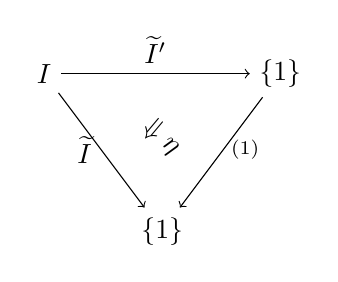
\begin{tikzpicture}
            % Define node positions
            \node (B) at (0, 2) {$I$}; \node (C) at (3, 2) {$\{ 1 \}$}; \node
            (A) at (1.5, 0) {$\{ 1 \}$};
            
            % Draw arrows
            \draw[->] (B) -- (C) node[midway, above] {$\widetilde{I}'$};
            \draw[->] (B) -- (A) node[midway, left] {$\widetilde{I}$}; \draw[->]
            (C) -- (A) node[midway, right] {$\id^{(1)}$};
            
            % Natural transformation arrow
            \node[rotate=-40] at (1.5, 1.2) {$\Downarrow \eta$};
            % \node at (1.7, 1.2) {$\eta$};
        \end{tikzpicture}
    \end{center}
    it holds:
    \[
        g = \gamma(f, \bar{g})
    \]

    This follows immediately from the op-fibration property, since
    we choose the color 
    \[
    \bigotimes_{i \in \widetilde{I}} X_i
    \]
    with its morphism $f$ to be a cocartesian lift of the morphism
    \[
        \langle n \rangle \overset{\widetilde{I}}{\to} \langle 1 \rangle
    \]
    in $\Brx$. The universal property is induced 
    by the universal property of the cocartesian morphism.
\end{rem}



\begin{const}\label{con:brx_monoidal} For the next part, let $\pi \colon
\Cotimes \to \Brx$ be a $\Brx$-monoidal category and we denote $\C \coloneqq
\Cotimes_{\langle 1 \rangle}$. In this construction we aim to define a braided
monoidal structure on $\C$. First, we introduce the following abuse of notation:
For a $2$-morphism $\eta$, i.e. a path between two configurations $c_1, c_2 \in
\E_2(n)$ in $\Brx$, we would write the following diagram below:
\begin{center}
    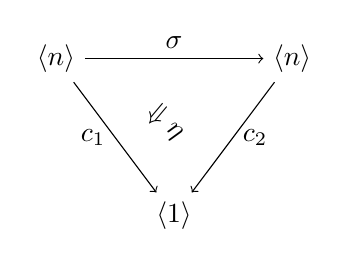
\begin{tikzpicture}
        % Define node positions
        \node (B) at (0, 2) {$\langle n \rangle$}; \node (C) at (3, 2) {$\langle
        n \rangle$}; \node (A) at (1.5, 0) {$\langle 1 \rangle$};
        % Draw arrows
        \draw[->] (B) -- (C) node[midway, above] {$\sigma$}; \draw[->] (B) --
        (A) node[midway, left] {$c_1$}; \draw[->] (C) -- (A) node[midway, right]
        {$c_2$};
        % Natural transformation arrow
        \node[rotate=-40] at (1.4, 1.2) {$\Downarrow \eta$};
        % \node at (1.7, 1.2) {$\eta$};
    \end{tikzpicture}
\end{center}

However, we use a slightly different notation for the sake of readability.
Instead, we write dashed arrows for the $2$-morphism as in the diagram:

\[    
    \begin{tikzcd}
        \langle n \rangle \arrow[r, "\sigma"] \arrow[d, "c_1"] & \langle n \rangle \arrow[d, "c_2"] \\
        \langle 1 \rangle  \arrow[r, dashed, "\eta"]                  & \langle 1 \rangle                
    \end{tikzcd}
\]


Let $\beta$ denote the following morphism in $\Brx$
     \begin{align*}
         \beta \colon \langle 2 \rangle &\to \langle 2 \rangle \\
         1 &\mapsto 2 \\
         2 &\mapsto 1 \\
     \end{align*}
with the trivial collection $(\id^2, \id^1)$. Further, let 
\begin{align*}
    \mu \colon \langle 2 \rangle &\to \langle 1 \rangle \\
    1 &\mapsto 1 \\
    2 &\mapsto 1 \\
\end{align*}
be the morphism with the basepoint configuration $b_2 \in \E_2(2)$:
\begin{center}
    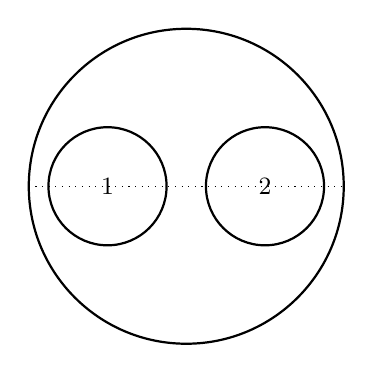
\begin{tikzpicture}
                        % First element (left)
                        \node at (1, 0) {\small $2$}; \node at (-1, 0) {\small
                        $1$};
                        
                        \draw[thick] (0,0) circle (2); \draw[thick] (1, 0)
                        circle (0.75); \draw[thick] (-1, 0) circle (0.75);
                        \draw[dotted](-2, 0)--(2, 0);       
        \end{tikzpicture}
\end{center}

Since $\pi$ satisfies the op-fibration condition (M1) and the Segal condition
(M2), we have that for any $(A,B) \in \C^2 \cong \Cotimes_{\langle 2 \rangle}$,
there is a cocartesian lift $(A,B) \to A \otimes B$ for $\mu \in \Brx$. The
cocartesian property ensures that the choice is unique up to unique isomorphism.
So, we obtain a well-defined functor:
\[
    \otimes \colon \C^2 \to \C.
\]

Further, we consider the following diagram in $\Brx$:
\[    
    \begin{tikzcd}
        \langle 2 \rangle \arrow[r, "\beta"] \arrow[d, "\mu"] & \langle 2 \rangle \arrow[d, "\mu"] \\
        \langle 1 \rangle  \arrow[r, dashed]                  & \langle 1 \rangle                
    \end{tikzcd}
\]
Note, that analogous to $\beta$ inducing $\otimes$, we obtain for $\otimes \circ
\beta$ a different functor:
\[
    \otimes' \colon \C^2 \to \C
\]
Filling the diagram, i.e. providing commutativity data, means choosing a homotopy
class of paths from the basepoint configuration, corresponding to $\mu$, to the
twisted basepoint configuration, corresponding to $\mu \circ \beta$. We choose
this to be the class of the half twist which we denote by $\htw$.

\begin{center}
    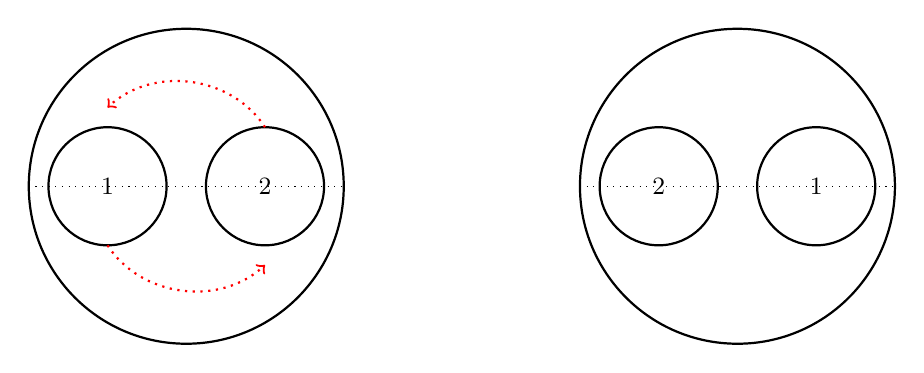
\begin{tikzpicture}
                        % basepoint
                        \node at (1, 0) {\small $2$}; \node at (-1, 0) {\small
                        $1$};
                        
                        \draw[thick] (0,0) circle (2); \draw[thick] (1, 0)
                        circle (0.75); \draw[thick] (-1, 0) circle (0.75);
                        \draw[dotted](-2, 0)--(2, 0); \draw[->, thick, dotted,
                        red] (-1, -0.75) to [bend right=50] (1, -1); \draw[->,
                        thick, dotted, red] (1, 0.75) to [bend right=50] (-1,
                        1);

                        \node at (3.5, 0) {$\rightsquigarrow$};
                        
                        % twisted basepoint
                        \node at (8, 0) {\small $1$}; \node at (6, 0) {\small
                        $2$};
                        
                        \draw[thick] (7,0) circle (2); \draw[thick] (8, 0)
                        circle (0.75); \draw[thick] (6, 0) circle (0.75);
                        \draw[dotted](5, 0)--(9, 0);  
                        
        \end{tikzpicture}
\end{center}

Since $\pi$ is an op-fibration, we obtain for a pair $(A,B)$ a cocartesian
morphism $$\beta' \colon (A,B) \to (B,A)$$ in $\C^2$ with $\pi(\beta')=\beta$.


Since $\otimes$ and $\beta'$ are cocartesian and composites of cocartesian
morphism are again cocartesian, we can lift the diagram for the class of the
half twist as well as for its inverse:
\[    
    \begin{tikzcd}
        \langle 2 \rangle \arrow[r, "\beta"] \arrow[d, "\mu"] & \langle 2 \rangle \arrow[d, "\mu"] \\
        \langle 1 \rangle  \arrow[r, dashed, shift left]                  & \langle 1 \rangle \arrow[l, dashed, shift left]                
    \end{tikzcd}
\]
Thus, we obtain two commuting diagrams in $\Cotimes$:
\[
\begin{tikzcd}
{(A,B)} \arrow[r, "\beta"] \arrow[d, "\otimes"] & {(B,A)} \arrow[d, "\otimes"]                        \\
A \otimes B \arrow[r, "b", dashed, shift left]  & B \otimes A \arrow[l, "b^{-1}", dashed, shift left]
\end{tikzcd}
\]
The morphism $b$ is induced by the cocartesian morphism $\otimes$
while $b^{-1}$ is induced by $\otimes \circ \beta'$. They are inverse to one
another since lifts with chosen source are unique and the identity is already a
lift. The induced morphism $b$ is a unique isomorphism due to the fact that
$\otimes$ and $\beta$ are cocartesian morphisms. Thus, we have defined a natural
isomorphism
\[
    \left\{b_{A,B} \colon A \otimes B \to B \otimes A\right\}_{(A,B) \in \C^2}.
\]
Note, that for a homotopically different choice of path instead of the half
twist, we would obtain a different braiding map. So, this choice is essential
for our construction.

We recall the following morphisms from $\Fin$ for $n \in \N$ and $1 \leq i \leq
n$:
\begin{align*}
    \tau^n_i \colon \langle n \rangle &\to \langle n-1 \rangle \\
    j &\mapsto \begin{cases}
        j &  1 \leq j \leq i \\
        j-1 & i < j \leq n \\
        \ast & j=\ast
    \end{cases}
\end{align*}
We consider these morphisms in $\Brx$ with the following collection of
configurations:
\begin{align*}
    \widetilde{\tau^n_i} \coloneq
     \begin{cases}
        b_2 &   i=j \\
        \id^j & \text{otherwise}
    \end{cases}
\end{align*}

For the associator we consider the following diagram in $\Brx$:
    \[
        \begin{tikzcd}
                                                                    & \langle 3 \rangle \arrow[ld, "\tau^3_2"'] \arrow[rd, "\tau^3_1"] &                                                               \\
            \langle 2 \rangle \arrow[d, "\mu"']                      &                                                                  & \langle 2 \rangle \arrow[d, "\mu"]                            \\
            \langle 1 \rangle \arrow[rr, "\eta", dashed, shift left] &                                                                  & \langle 1 \rangle \arrow[ll, "\eta^{-1}", dashed, shift left]
        \end{tikzcd}
    \]
    To fill the diagram, we choose a homotopy class of paths $\eta$ that only
    translates the middle points of the disks along the horizontal line and
    shrinks or expands the disks as needed. This is an $\E_1$-translation as
    defined in Remark \ref{rem:e1-translation} and is therefore unique as such.
    \begin{center}
        \begin{tikzpicture}
                        % First element (left)
                        \node at (-1, 0) {\small $1$}; \node at (0.625, 0)
                        {\small $2$}; \node at (1.375, 0) {\small $3$};
                        \draw[thick] (0,0) circle (2); \draw[thick] (-1, 0)
                        circle (0.75); \draw[thick] (0.625, 0) circle (0.275);
                        \draw[thick] (1.375, 0) circle (0.275); \draw[dotted]
                        (1, 0) circle (0.75); \draw[dotted](-2, 0)--(2, 0);

                        \node at (3.5, 0) {$\overset{\eta}{\rightsquigarrow}$};

                        % Second element (left)
                        \node at (5.625, 0) {\small  $1$}; \node at (6.375, 0)
                        {\small $2$}; \node at (8, 0) {\small$3$}; \draw[thick]
                        (7,0) circle (2); \draw[dotted] (6, 0) circle (0.75);
                        \draw[thick] (6.325, 0) circle (0.275); \draw[thick]
                        (5.675, 0) circle (0.275); \draw[thick] (8, 0) circle
                        (0.75); \draw[dotted](5, 0)--(9, 0);     
        \end{tikzpicture}
    \end{center}

Again using the op-fibration condition (M1) property of $\pi$ we obtain a
commuting diagram in $\Cotimes$:
\[
    \begin{tikzcd}
        {(A \otimes B, C)} \arrow[d, "\otimes"] & {(A,B,C)} \arrow[r, "{(\id, \otimes)}"] \arrow[l, "{(\otimes, \id)}"'] & {(A, B \otimes C)} \arrow[d, "\otimes"] \\
        (A \otimes B) \otimes C \arrow[rr, "a", shift left] &                                                                        & A \otimes (B \otimes C) \arrow[ll, "a^{-1}", shift left]                
    \end{tikzcd}
\]

Similarily to Proposition \ref{SymMonBijection}, the tensor unit is given by the
unique morphism $\eta \colon \langle 0 \rangle \to \langle 1 \rangle$ in $\Brx$
which induces a functor $\Cotimes_{\langle 0 \rangle} \to \C$ giving us a tensor
unit $\mathbf{1}$.
\end{const}

\begin{prop}\label{prop:braidmon} The category $\C$ equipped with $(\otimes, b,
    a, \mathbf{1})$ as in Construction \ref{con:brx_monoidal} defines a braided
    monoidal category.
\end{prop}

\begin{proof}
    % First, we observe that the associator refers to $\E_1$ being embedded into
    % $\E_2$ along the horizontal line, as we translate and resize the disks
    % along the horizontal line. So, we can arbitrarly translate and resize
    % configurations with middle points on the horizontal axis, since it is only
    % a associative translation in $\E_1$. 

    % \begin{figure}[h!] \begin{center} \begin{tikzpicture} \draw[dotted]
    %     (-13,0) -- (-9,0); \draw[thick, red] (-12.75,0) -- (-11.25,0);
    %     \draw[thick, orange] (-10.6,0) -- (-10.05,0); \draw[thick, purple]
    %     (-9.95,0) -- (-9.4,0);

    %             % configuration in #E2
    %             \draw[dotted] (-7,0) -- (-3,0);
    %             \draw[thick] (-5,0) circle (2);
    %             \draw[thick, red] (-6, 0) circle (0.75);
    %             \draw[thick, orange] (-4.325, 0) circle (0.275);
    %             \draw[thick, purple] (-3.675, 0) circle (0.275);
    %             % \node at (-6.25, 0) {\small $1$};
    %             % \node at (-5, 0) {\small $2$};
    %             % \node at (-3.75, 0) {\small $3$};  
    %             \node at (-8, 0) {$\hookrightarrow$}; 
    %         \end{tikzpicture}
    %     \end{center}
    %     \caption{example of a configuration of $\E_1$ being embedded in $\E_2$ along the horizontal line}
    % \end{figure}

    First, the pentagon identity holds as compositions of $\E_1$-translations
    are $\E_1$-translations and are unique up to homotopy. The unitality
    condition holds analogously to the proof of Proposition
    \ref{SymMonBijection} using the Segal condition. Hence, we focus on
    verifying the hexagon identities:
    \begin{enumerate}
        \item 
        \[
            \begin{tikzcd}
                                                                                & A \otimes (B \otimes C) \arrow[r, "b"] & (B \otimes C) \otimes A  \arrow[rd, "a"]            &                         \\
            (A \otimes B) \otimes C \arrow[ru, "a"] \arrow[rd, "b \otimes \id"] &                                        &                                                     & B \otimes (C \otimes A) \\
                                                                                & (B \otimes A) \otimes C \arrow[r, "a"] & B \otimes (A \otimes C) \arrow[ru, "\id \otimes b"] &                        
            \end{tikzcd}
        \]
        \item 
        \[
            \begin{tikzcd}
                                                                                & (A \otimes B) \otimes C \arrow[r, "b"] & C \otimes (A \otimes B) \arrow[rd, "a"]             &                         \\
            A \otimes (B \otimes C) \arrow[ru, "a"] \arrow[rd, "\id \otimes b"] &                                        &                                                     & (C \otimes A) \otimes B \\
                                                                                & A \otimes (C \otimes B) \arrow[r, "a"] & (A \otimes C) \otimes B \arrow[ru, "b \otimes \id"] &                        
            \end{tikzcd}
        \]
    \end{enumerate}
    Each edge in the hexagon diagrams refers to a commuting diagram in $\Brx$ of
    the form

    \[
        \begin{tikzcd}
                                            & \langle 3 \rangle \arrow[ldd, "c_{A \otimes B \otimes C}"', bend right] \arrow[d, "c_{(A \otimes B) \otimes C}" description] \arrow[rdd, "c_{C \otimes (A\otimes B)}", bend left] &                   \\
                                            & \langle 1 \rangle \arrow[ld, dashed] \arrow[rd, dashed]                                                                                                                            &                   \\
        \langle 1 \rangle \arrow[rr, dashed] &                                                                                                                                                                                   & \langle 1 \rangle
        \end{tikzcd}
    \]
   
    with configurations:
    \begin{center}
        \begin{adjustbox}{max height= 4cm}
        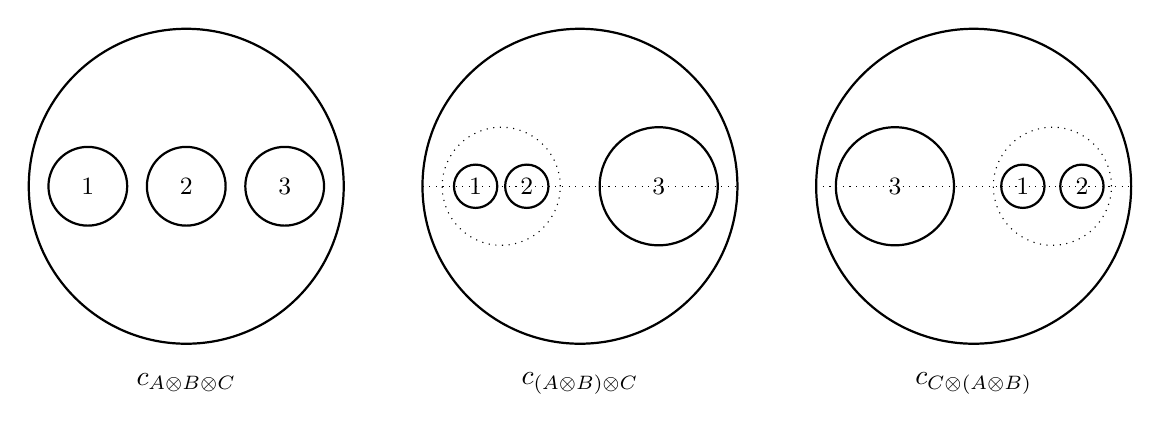
\begin{tikzpicture}
            \node at (0,-2.5) {$c_{(A \otimes B) \otimes C}$}; \node at
            (-5,-2.5) {$c_{A \otimes B \otimes C}$}; \node at (5,-2.5) {$c_{C
            \otimes (A \otimes B)}$};


            % left configuration (left)
            \draw[thick] (-5,0) circle (2); \draw[thick] (-3.75, 0) circle
            (0.5); \draw[thick] (-5, 0) circle (0.5); \draw[thick] (-6.25, 0)
            circle (0.5); \node at (-6.25, 0) {\small $1$}; \node at (-5, 0)
            {\small $2$}; \node at (-3.75, 0) {\small $3$};

            % second configuration (middle)
            \node at (-0.675, 0) {\small $2$}; \node at (-1.325, 0) {\small
            $1$}; \node at (1, 0) {\small $3$}; \draw[thick] (0,0) circle (2);
            \draw[dotted] (-1, 0) circle (0.75); \draw[thick] (-0.675, 0) circle
            (0.275); \draw[thick] (-1.325, 0) circle (0.275); \draw[thick] (1,
            0) circle (0.75); \draw[dotted](-2, 0)--(2, 0);

            % third element (right)
            \node at (4, 0) {\small $3$}; \node at (5.625, 0) {\small $1$};
            \node at (6.375, 0) {\small $2$}; \draw[thick] (5,0) circle (2);
            \draw[thick] (4, 0) circle (0.75); \draw[thick] (5.625, 0) circle
            (0.275); \draw[thick] (6.375, 0) circle (0.275); \draw[dotted] (6,
            0) circle (0.75); \draw[dotted](3, 0)--(7, 0);  
        \end{tikzpicture}
        \end{adjustbox}
    \end{center}
    % \todo{describe one commuting tetrahedron in detail. Rest analogpously
    % leading tot he following diagram...}
    The commutativity of the triangle diagrams on the side means choosing a path
    as representative of a homotopy class of paths from one configuration to
    another, while filling the tetrahedron in $\Brx$ means verifying that the
    paths are from the same homotopy class, i.e. there exists a homotopy between
    the paths. As it turns out we do not make any new choices of paths. The
    paths are induced by the half twist $\htw$ we chose to define $\otimes$.

    Let us understand where the diagram, or more precisely the configurations
    come from. The morphisms corresponding to $c_{(A \otimes B) \otimes C}$ and
    $c_{C \otimes (A \otimes B)}$ respectively factor through $\langle 2
    \rangle$ in the following way:
    \begin{center}
        \begin{tikzcd}
                                                & \langle 3 \rangle \arrow[ldd,
                                                "c_{(A \otimes B) \otimes C}"',
                                                bend right] \arrow[rdd, "c_{C
                                                \otimes (A \otimes B)}", bend
                                                left] \arrow[d, "\tau_2^3"] & \\
                                                & \langle 2 \rangle \arrow[ld,
                                                "\mu"'] \arrow[rd, "\mu \circ
                                                \beta"] &                   \\
            \langle 1 \rangle \arrow[rr, "\htw", dashed] & & \langle 1 \rangle
        \end{tikzcd}
    \end{center}
    We observe, that the outer triangle commutes precisely because the inner
    triangle commutes which is the case, since we already chose the path to be
    the half twist $\htw$.
    \begin{center}
    \begin{adjustbox}{max height= 3cm}
    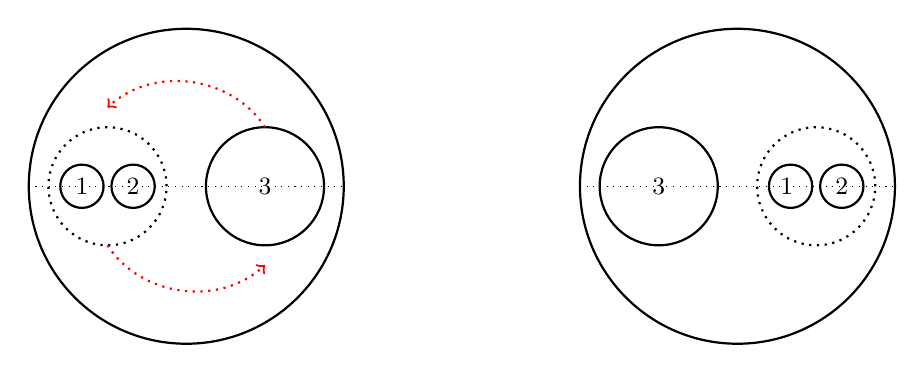
\begin{tikzpicture}
                        % basepoint
                        \node at (1, 0) {\small $3$}; \node at (-1.325, 0)
                        {\small $1$}; \node at (-0.675, 0) {\small $2$};
                        
                        \draw[thick] (0,0) circle (2); \draw[thick] (1, 0)
                        circle (0.75); \draw[thick, dotted] (-1, 0) circle
                        (0.75); \draw[thick] (-0.675, 0) circle (0.275);
                        \draw[thick] (-1.325, 0) circle (0.275);
                        \draw[dotted](-2, 0)--(2, 0); \draw[->, thick, dotted,
                        red] (-1, -0.75) to [bend right=50] (1, -1); \draw[->,
                        thick, dotted, red] (1, 0.75) to [bend right=50] (-1,
                        1);

                        \node at (3.5, 0) {$\rightsquigarrow$};
                        
                        % twisted basepoint
                        \node at (7.625, 0) {\small $1$}; \node at (8.325, 0)
                        {\small $2$}; \node at (6, 0) {\small $3$};
                        
                        \draw[thick] (7,0) circle (2); \draw[thick, dotted] (8,
                        0) circle (0.75); \draw[thick] (6, 0) circle (0.75);
                        \draw[thick] (7.675, 0) circle (0.275); \draw[thick]
                        (8.325, 0) circle (0.275); \draw[dotted](5, 0)--(9, 0);  
        \end{tikzpicture}
    \end{adjustbox}
    \end{center}

    Similar arguments for all the corresponding diagrams induced by the hexagon
    identity $(1)$ give us paths that are already defined by the associativity
    path $\eta$ and the half twist $\htw$.
    \begin{center}
        \begin{adjustbox}{max height= 16cm}
        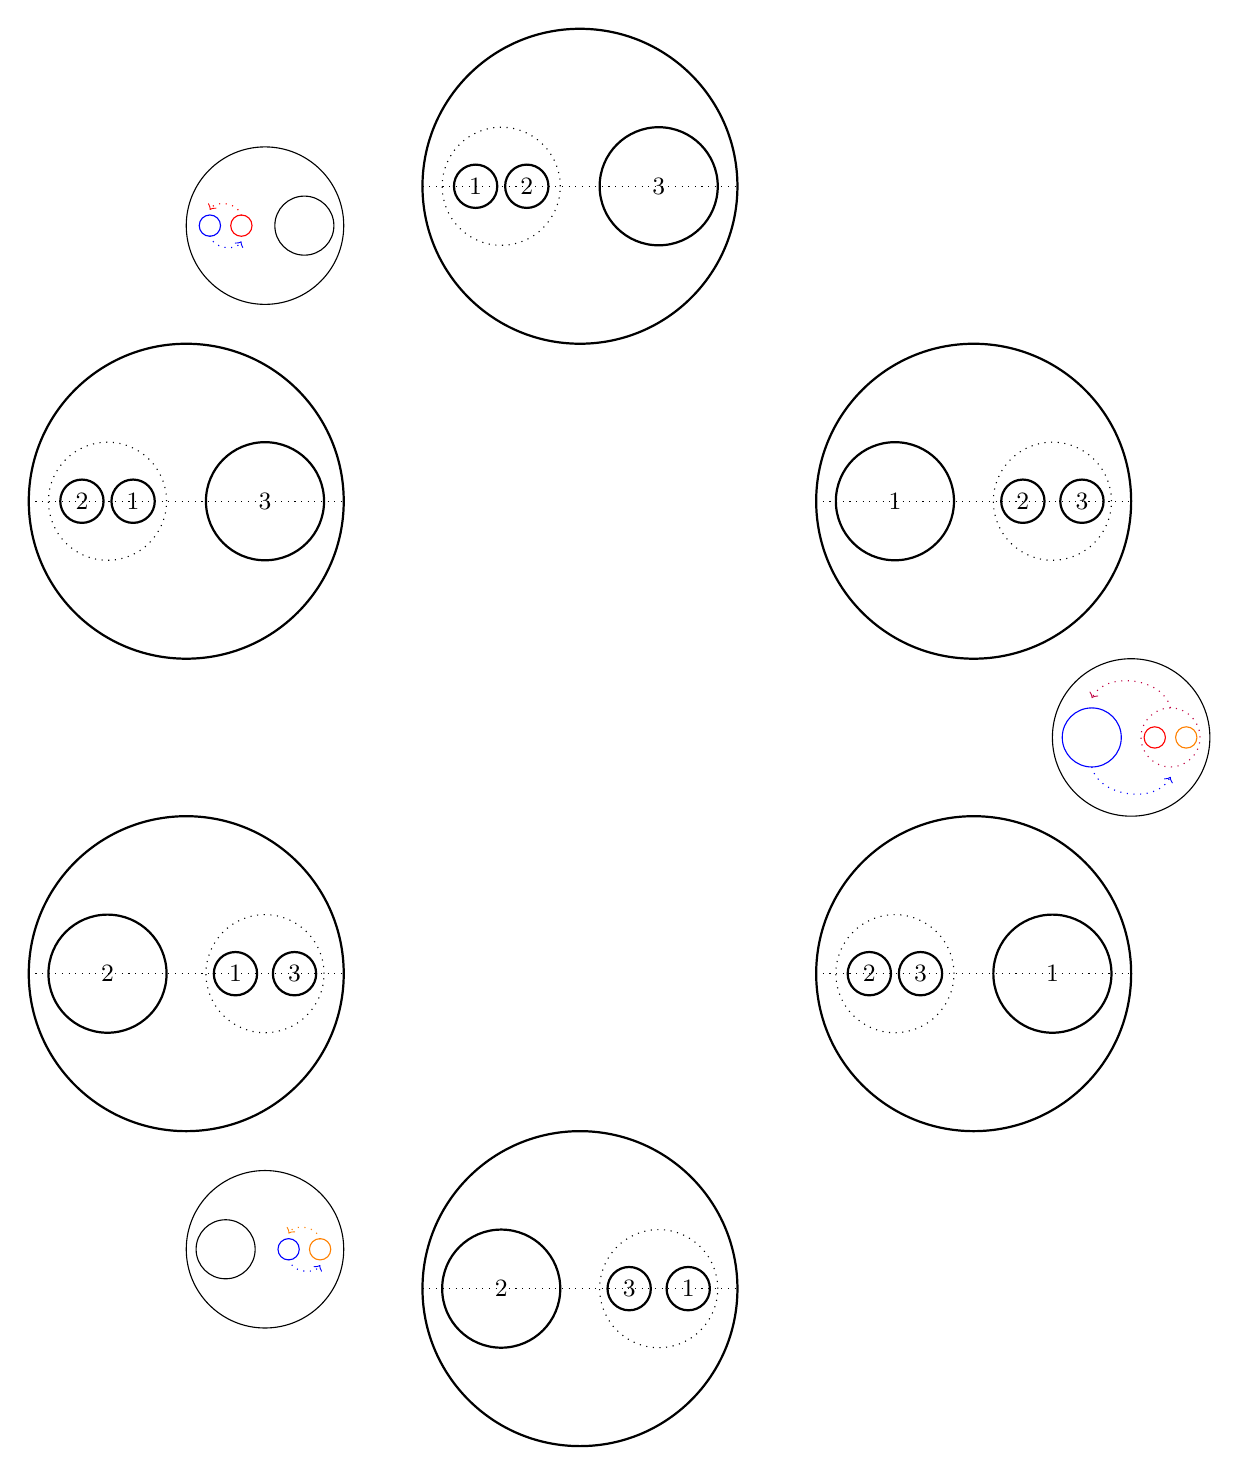
\begin{tikzpicture}
            %arrows
            \node at (-2.5, -2) {\rotatebox{-135}{$\rightsquigarrow$}}; \node at
            (2.5, -2) {\rotatebox{-45}{$\rightsquigarrow$}}; \node at (-5, -7)
            {\rotatebox{-90}{$\rightsquigarrow$}}; \node at (5, -7)
            {\rotatebox{-90}{$\rightsquigarrow$}}; \node at (2.5, -12)
            {\rotatebox{-135}{$\rightsquigarrow$}}; \node at (-2.5, -12)
            {\rotatebox{-45}{$\rightsquigarrow$}};

            % top
            \node at (-0.675, 0) {\small $2$}; \node at (-1.325, 0) {\small
            $1$}; \node at (1, 0) {\small $3$}; \draw[thick] (0,0) circle (2);
            \draw[dotted] (-1, 0) circle (0.75); \draw[thick] (-0.675, 0) circle
            (0.275); \draw[thick] (-1.325, 0) circle (0.275); \draw[thick] (1,
            0) circle (0.75); \draw[dotted](-2, 0)--(2, 0);

            % right first
            \node at (4, -4) {\small $1$}; \node at (5.625, -4) {\small $2$};
            \node at (6.375, -4) {\small $3$}; \draw[thick] (5,-4) circle (2);
            \draw[thick] (4, -4) circle (0.75); \draw[thick] (5.625, -4) circle
            (0.275); \draw[thick] (6.375, -4) circle (0.275); \draw[dotted] (6,
            -4) circle (0.75); \draw[dotted](3, -4)--(7, -4); 
                 
            % left first
            \node at (-5.675, -4) {\small $1$}; \node at (-6.325, -4) {\small
            $2$}; \node at (-4, -4) {\small $3$}; \draw[thick] (-5,-4) circle
            (2); \draw[dotted] (-6, -4) circle (0.75); \draw[thick] (-5.675, -4)
            circle (0.275); \draw[thick] (-6.325, -4) circle (0.275);
            \draw[thick] (-4, -4) circle (0.75); \draw[dotted](-7, -4)--(-3,
            -4);

            % right second
            \node at (4.325, -10) {\small $3$}; \node at (3.675, -10) {\small
            $2$}; \node at (6, -10) {\small $1$}; \draw[thick] (5,-10) circle
            (2); \draw[dotted] (4, -10) circle (0.75); \draw[thick] (4.325, -10)
            circle (0.275); \draw[thick] (3.675, -10) circle (0.275);
            \draw[thick] (6, -10) circle (0.75); \draw[dotted](3, -10)--(7,
            -10);

            % left second
            \node at (-6, -10) {\small $2$}; \node at (-4.375, -10) {\small
            $1$}; \node at (-3.625, -10) {\small $3$}; \draw[thick] (-5,-10)
            circle (2); \draw[thick] (-6, -10) circle (0.75); \draw[thick]
            (-4.375, -10) circle (0.275); \draw[thick] (-3.625, -10) circle
            (0.275); \draw[dotted] (-4, -10) circle (0.75); \draw[dotted](-7,
            -10)--(-3, -10);

            %bottom
            \node at (-1, -14) {\small $2$}; \node at (0.625, -14) {\small $3$};
            \node at (1.375, -14) {\small $1$}; \draw[thick] (0,-14) circle (2);
            \draw[thick] (-1, -14) circle (0.75); \draw[thick] (0.625, -14)
            circle (0.275); \draw[thick] (1.375, -14) circle (0.275);
            \draw[dotted] (1, -14) circle (0.75); \draw[dotted](-2, -14)--(2,
            -14);

            % paths visualisation #1
            \draw (-4,-0.5) circle (1);
            %\draw[dotted] (-1, 0) circle (0.375);
            \draw[blue] (-4.7, -0.5) circle (0.13525); \draw[red] (-4.3, -0.5)
            circle (0.13525); \draw (-3.5, -0.5) circle (0.375); \draw[->,
            dotted, red] (-4.3, -0.375) to [bend right=70] (-4.7, -0.3);
            \draw[->, dotted, blue] (-4.7, -0.625) to [bend right=70] (-4.3,
            -0.7);

            % paths visualisation #2
            \draw (-4,-13.5) circle (1);
            %\draw[dotted] (-1, 0) circle (0.375);
            \draw[orange] (-3.3, -13.5) circle (0.13525); \draw[blue] (-3.7,
            -13.5) circle (0.13525); \draw (-4.5, -13.5) circle (0.375);
            \draw[->, dotted, blue] (-3.7, -13.625) to [bend right=70] (-3.3,
            -13.7); \draw[->, dotted, orange] (-3.3, -13.375) to [bend right=70]
            (-3.7, -13.3);

            % paths visualisation #3
            \draw (7,-7) circle (1); \draw[dotted, purple] (7.5, -7) circle
            (0.375); \draw[orange] (7.7, -7) circle (0.13525); \draw[red] (7.3,
            -7) circle (0.13525); \draw[blue] (6.5, -7) circle (0.375);
            \draw[->, dotted, purple] (7.5, -6.625) to [bend right=70] (6.5,
            -6.5); \draw[->, dotted, blue] (6.5, -7.375) to [bend right=70]
            (7.5, -7.5);
        \end{tikzpicture}
        \end{adjustbox}
    \end{center}

        The resulting paths are the following representatives of their homotopy
    class and they are clearly homotopy equivalent. 

    \begin{center}
        \begin{adjustbox}{max height= 3cm}
        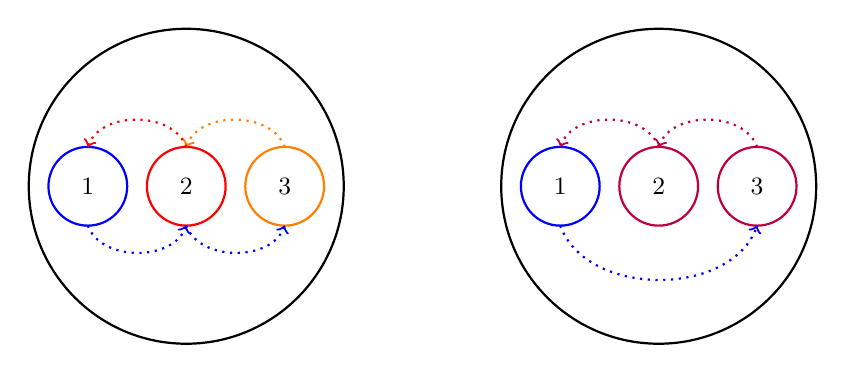
\begin{tikzpicture}
            %arrow
            \node at (-2, -0) {$\rightsquigarrow$};

            % left side paths
            \draw[thick] (-5,0) circle (2); \draw[thick, orange] (-3.75, 0)
            circle (0.5); \draw[thick, red] (-5, 0) circle (0.5); \draw[thick,
            blue] (-6.25, 0) circle (0.5); \node at (-6.25, 0) {\small $1$};
            \node at (-5, 0) {\small $2$}; \node at (-3.75, 0) {\small $3$};

            %right side paths
            \draw[thick] (1,0) circle (2); \draw[thick, purple] (2.25, 0) circle
            (0.5); \draw[thick, purple] (1, 0) circle (0.5); \draw[thick, blue]
            (-0.25, 0) circle (0.5); \node at (-0.25, 0) {\small $1$}; \node at
            (1, 0) {\small $2$}; \node at (2.25, 0) {\small $3$};

            % paths
            \draw[->, dotted, thick, orange] (-3.75, 0.5) to [bend right=70]
            (-5, 0.5); \draw[->, dotted, thick, red] (-5, 0.5) to [bend
            right=70] (-6.25, 0.5); \draw[->, dotted, thick, blue] (-6.25, -0.5)
            to [bend right=70] (-5, -0.5); \draw[->, dotted, thick, blue] (-5,
            -0.5) to [bend right=70] (-3.75, -0.5); \draw[->, dotted, thick,
            purple] (2.25, 0.5) to [bend right=70] (1, 0.5); \draw[->, dotted,
            thick, purple] (1, 0.5) to [bend right=70] (-0.25, 0.5); \draw[->,
            dotted, thick, blue] (-0.25, -0.5) to [bend right=70] (2.25, -0.5);
        \end{tikzpicture}
        \end{adjustbox}
    \end{center}

    Analogously for the hexagon identity $(2)$, we consider the composition of
    $2$-morphism in $\Brx$:

    \begin{center}
        \begin{adjustbox}{max height= 16cm}
        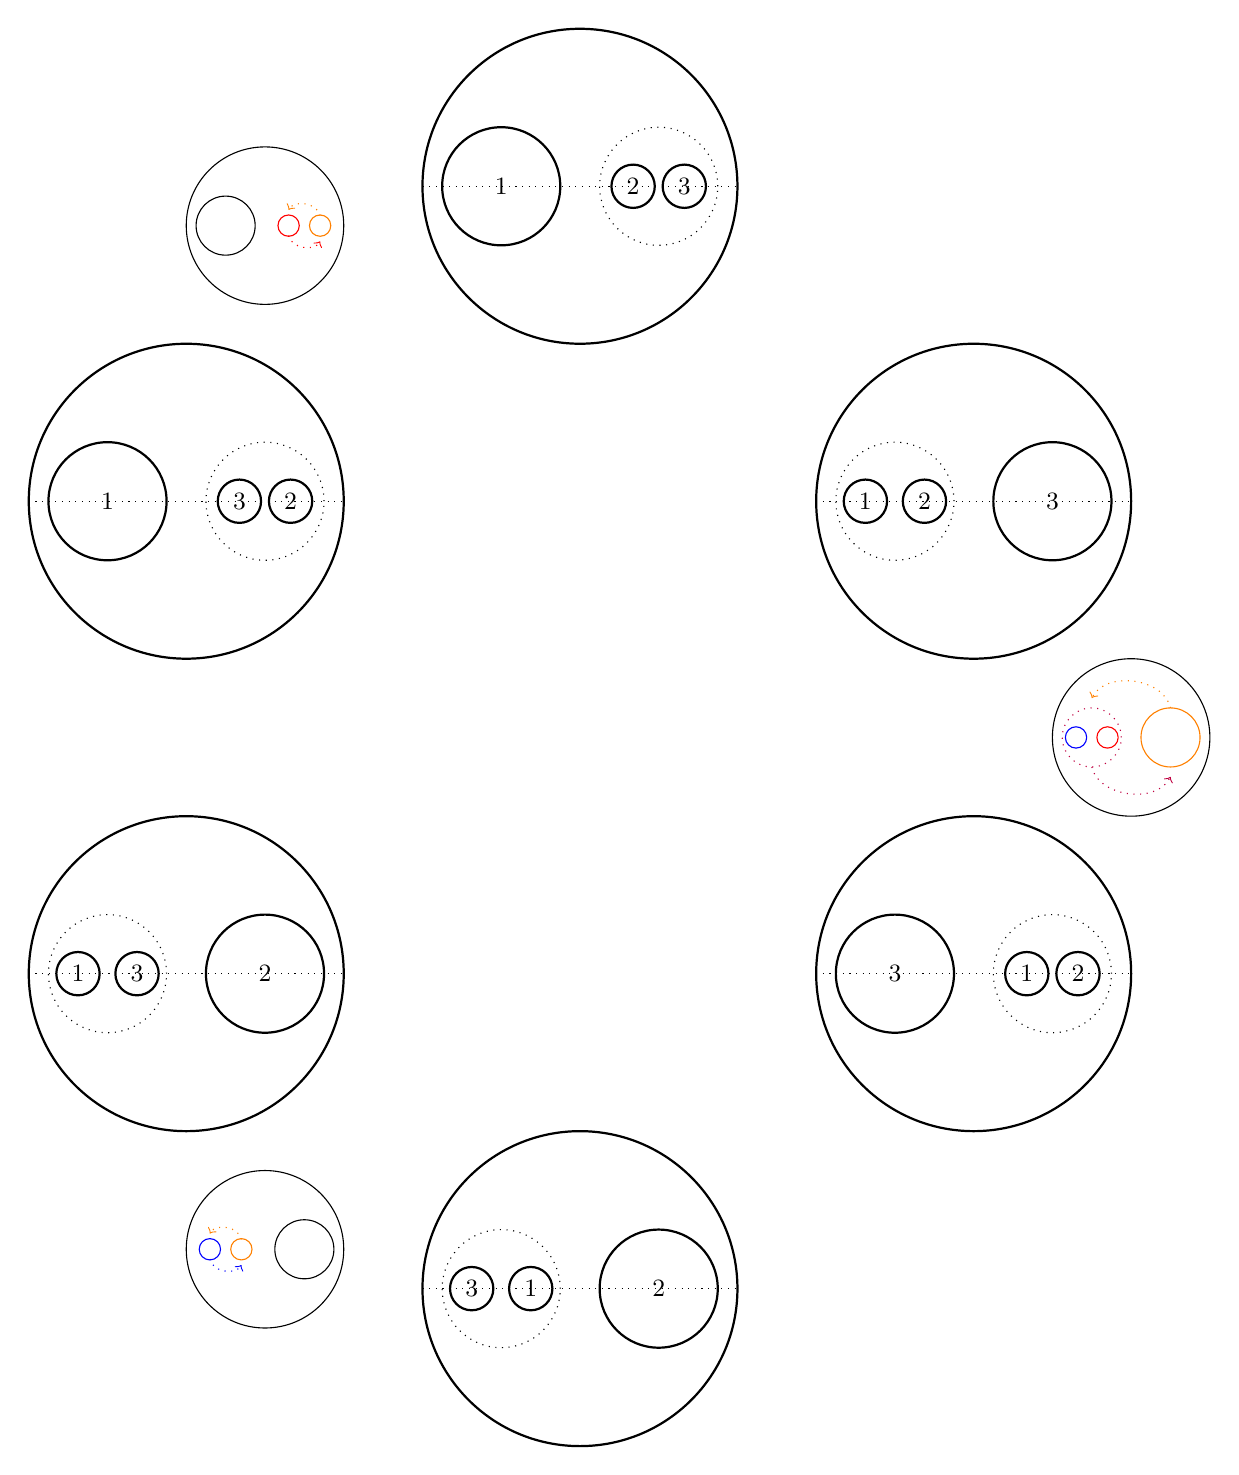
\begin{tikzpicture}
            %arrows
            \node at (-2.5, -2) {\rotatebox{-135}{$\rightsquigarrow$}}; \node at
            (2.5, -2) {\rotatebox{-45}{$\rightsquigarrow$}}; \node at (-5, -7)
            {\rotatebox{-90}{$\rightsquigarrow$}}; \node at (5, -7)
            {\rotatebox{-90}{$\rightsquigarrow$}}; \node at (2.5, -12)
            {\rotatebox{-135}{$\rightsquigarrow$}}; \node at (-2.5, -12)
            {\rotatebox{-45}{$\rightsquigarrow$}};

            % top
            \node at (0.675, 0) {\small $2$}; \node at (1.325, 0) {\small $3$};
            \node at (-1, 0) {\small $1$}; \draw[thick] (0,0) circle (2);
            \draw[dotted] (1, 0) circle (0.75); \draw[thick] (0.675, 0) circle
            (0.275); \draw[thick] (1.325, 0) circle (0.275); \draw[thick] (-1,
            0) circle (0.75); \draw[dotted](-2, 0)--(2, 0);

            % right first
            \node at (6, -4) {\small $3$}; \node at (3.625, -4) {\small $1$};
            \node at (4.375, -4) {\small $2$}; \draw[thick] (5,-4) circle (2);
            \draw[thick] (6, -4) circle (0.75); \draw[thick] (3.625, -4) circle
            (0.275); \draw[thick] (4.375, -4) circle (0.275); \draw[dotted] (4,
            -4) circle (0.75); \draw[dotted](3, -4)--(7, -4); 
                 
            % left first
            \node at (-3.675, -4) {\small $2$}; \node at (-4.325, -4) {\small
            $3$}; \node at (-6, -4) {\small $1$}; \draw[thick] (-5,-4) circle
            (2); \draw[dotted] (-4, -4) circle (0.75); \draw[thick] (-3.675, -4)
            circle (0.275); \draw[thick] (-4.325, -4) circle (0.275);
            \draw[thick] (-6, -4) circle (0.75); \draw[dotted](-7, -4)--(-3,
            -4);

            % right second
            \node at (6.325, -10) {\small $2$}; \node at (5.675, -10) {\small
            $1$}; \node at (4, -10) {\small $3$}; \draw[thick] (5,-10) circle
            (2); \draw[dotted] (6, -10) circle (0.75); \draw[thick] (6.325, -10)
            circle (0.275); \draw[thick] (5.675, -10) circle (0.275);
            \draw[thick] (4, -10) circle (0.75); \draw[dotted](3, -10)--(7,
            -10);

            % left second
            \node at (-4, -10) {\small $2$}; \node at (-6.375, -10) {\small
            $1$}; \node at (-5.625, -10) {\small $3$}; \draw[thick] (-5,-10)
            circle (2); \draw[thick] (-4, -10) circle (0.75); \draw[thick]
            (-6.375, -10) circle (0.275); \draw[thick] (-5.625, -10) circle
            (0.275); \draw[dotted] (-6, -10) circle (0.75); \draw[dotted](-7,
            -10)--(-3, -10);

            %bottom
            \node at (1, -14) {\small $2$}; \node at (-0.625, -14) {\small $1$};
            \node at (-1.375, -14) {\small $3$}; \draw[thick] (0,-14) circle
            (2); \draw[thick] (1, -14) circle (0.75); \draw[thick] (-0.625, -14)
            circle (0.275); \draw[thick] (-1.375, -14) circle (0.275);
            \draw[dotted] (-1, -14) circle (0.75); \draw[dotted](-2, -14)--(2,
            -14);

            % paths visualisation #1
            \draw (-4,-0.5) circle (1);
            %\draw[dotted] (-1, 0) circle (0.375);
            \draw[red] (-3.7, -0.5) circle (0.13525); \draw[orange] (-3.3, -0.5)
            circle (0.13525); \draw (-4.5, -0.5) circle (0.375); \draw[->,
            dotted, orange] (-3.3, -0.375) to [bend right=70] (-3.7, -0.3);
            \draw[->, dotted, red] (-3.7, -0.625) to [bend right=70] (-3.3,
            -0.7);

            % paths visualisation #2
            \draw (-4,-13.5) circle (1);
            %\draw[dotted] (-1, 0) circle (0.375);
            \draw[orange] (-4.3, -13.5) circle (0.13525); \draw[blue] (-4.7,
            -13.5) circle (0.13525); \draw (-3.5, -13.5) circle (0.375);
            \draw[->, dotted, blue] (-4.7, -13.625) to [bend right=70] (-4.3,
            -13.7); \draw[->, dotted, orange] (-4.3, -13.375) to [bend right=70]
            (-4.7, -13.3);

            % paths visualisation #3
            \draw (7,-7) circle (1); \draw[dotted, purple] (6.5, -7) circle
            (0.375); \draw[red] (6.7, -7) circle (0.13525); \draw[blue] (6.3,
            -7) circle (0.13525); \draw[orange] (7.5, -7) circle (0.375);
            \draw[->, dotted, purple] (6.5, -7.375) to [bend right=70] (7.5,
            -7.5); \draw[->, dotted, orange] (7.5, -6.625) to [bend right=70]
            (6.5, -6.5);
        \end{tikzpicture}
        \end{adjustbox}
    \end{center}

    The resulting paths are the following representatives of their homotopy
    class and they are homotopy equivalent. Therefore, the second hexagon
    identity holds.
    \begin{center}
        \begin{adjustbox}{max height= 3cm}
        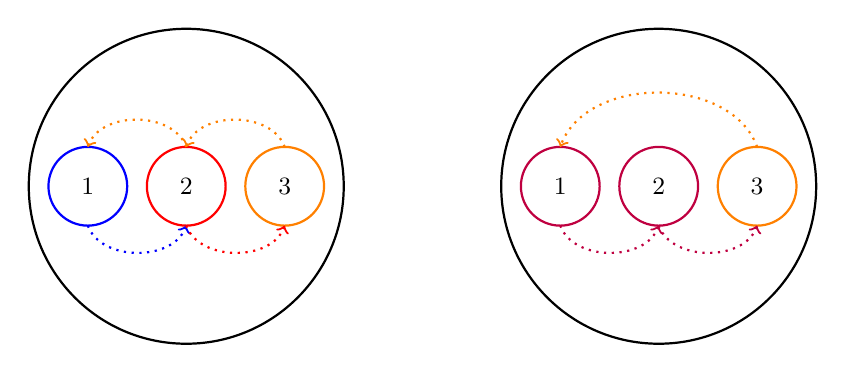
\begin{tikzpicture}
            %arrows
            \node at (-2, -0) {$\rightsquigarrow$};

            % left side paths
            \draw[thick] (-5,0) circle (2); \draw[thick, orange] (-3.75, 0)
            circle (0.5); \draw[thick, red] (-5, 0) circle (0.5); \draw[thick,
            blue] (-6.25, 0) circle (0.5); \node at (-6.25, 0) {\small $1$};
            \node at (-5, 0) {\small $2$}; \node at (-3.75, 0) {\small $3$};

            %right side paths
            \draw[thick] (1,0) circle (2); \draw[thick, orange] (2.25, 0) circle
            (0.5); \draw[thick, purple] (1, 0) circle (0.5); \draw[thick,
            purple] (-0.25, 0) circle (0.5); \node at (-0.25, 0) {\small $1$};
            \node at (1, 0) {\small $2$}; \node at (2.25, 0) {\small $3$};

            % paths
            \draw[->, dotted, thick, orange] (-3.75, 0.5) to [bend right=70]
            (-5, 0.5); \draw[->, dotted, thick, orange] (-5, 0.5) to [bend
            right=70] (-6.25, 0.5); \draw[->, dotted, thick, blue] (-6.25, -0.5)
            to [bend right=70] (-5, -0.5); \draw[->, dotted, thick, red] (-5,
            -0.5) to [bend right=70] (-3.75, -0.5); \draw[->, dotted, thick,
            purple]  (1, -0.5) to [bend right=70] (2.25, -0.5); \draw[->,
            dotted, thick, purple]  (-0.25, -0.5) to [bend right=70] (1, -0.5);
            \draw[->, dotted, thick, orange]  (2.25, 0.5) to [bend right=70]
            (-0.25, 0.5);
        \end{tikzpicture}
    \end{adjustbox}
    \end{center}
    This concludes the proof that $\Brx$ induces a braided monoidal structure on
    $\C$.

\end{proof}
